\documentclass{article}
\usepackage{url}
\usepackage{algpseudocode}
\usepackage{verbatim}
\usepackage{microtype}
\usepackage{enumerate}
\usepackage{enumitem}
\usepackage{epsfig}
\usepackage{algorithmicx}
\usepackage{algorithm}
\usepackage{authblk}
\usepackage{caption}
\usepackage{lscape}
\begin{document}

\title{Finding Bots and Spammers on Wikipedia}


\author[1]{Sarah Weissman (sew@umd.edu)}
\affil[1]{University of Maryland, College of Information Studies}

\date{August 16, 2013}

\maketitle
\begin{abstract}
\end{abstract}

\section{Introduction}

Wikipedia is an open-source collaboratively edited encyclopedia. It is viewable and editable by anyone, with editing changes viewable immediately. Although Wikipedia is not a social network, Collaborative editing on Wikipedia has its social aspects. Although it is possible to edit Wikipedia anonymously, or to merely view Wikipedia without editing at all, many Wikipedia editors create user accounts. User accounts have associated User pages. Although these pages are not profiles (link to Wikipedia policy), they are spaces in which user-to-user communication takes place and serve as a scratch space where users can work on drafts of articles. Many editors organize themselves around communities (projects?) focused on editing or expanding Wikipedia content on specific topics or on other Wikipedia adminstistrative editing tasks. (Examples of communities?)

In this paper we use techniques from social network analysis to attempt to identify certain types of user behaviour on Wikipedia. Specifically we are interested in identifying bots and spammers. Although the behaviour of bots and spammers might be considered anti-social, rather than social, the ability to identify them can benefit social nework analysis of Wikipedia in several ways. Filtering out such users can give a more balanced view of the network of Wikipedia editors. Although bots are allowed on Wikipedia and serve an important purpose, since they have the potential to make many more edits to many more articles in a short period of time than a human user, their behavior can make their editing contributions look more significant than it actually is to a network. Spammers are useful to detect, since their behavior is undesirable and if detected could be automatically stopped. Spammers may also clutter up the network by editing anonymously and unpredictably.

Define spammers and bots more precisely.

Techniques for big data processing make it easier to get a big picture of the Wikipedia network of editors. We take advantage of the MapReduce to process user data.

\section{Related Work}
%    Related work - a literature review of papers on similar topics

There have been many studies of the social nature of wikipedia editing. Most research focuses on a dynamic analysis where changes in the edit graph are viewed over time or for a specific window of time around a particular event. However, many of the newest and most comprehensive studies of collaborative Wikipedia editing use older data sets (most often data from 2006/2007).

Iba, et al. (2010) use ``dynamic social network analyssis'' to analyze editing patterns of Wikipedia contributors to 2580 featured articles from English Wikipedia. They identify two categories of edotrs, coolfarmers and egoboosters. Coolfarmers are prolific editors who create original content, often focusing on things that are ``cool'' or newsworthy. Egoboosters spend most of their time ``polishing their own profile.'' Since Wikipedia editors do not have a personal profile page, it is unclear whether Egoboosters are editors who write Wikipedia articles about themselves, or who mostly post on their on User namespace page. Iba, et al. suggest that coolfarming behavior can be characterized using high betweenness centrality in the edit graph around the time period in which an article is being created, but do not develop specific criteria for identifying such user behavior.

West, et. al (2010) build a classifier to detect vandalism on Wikipedia for a years worth of edits, using a number of simple and aggregate features such as IP address, time since user registration, time of last edit, and reision comment length. They take advantage of use ``time-delayed behavioral observations'' and use edit reversion to define their data set for modeling.

Welser, et. al (2011) use structural signatures of egocentric networks to identify four key roles of Wikipedia editors: substantive experts, technical editors, vandal fighters and social networkers (122). Using a combination of hand picked accounts. Distribution across namespaces. They use data from 2006 to build a user network based on edits to the User:Talk namespace. Although they profile highly prolific editors, they do not distinguish bot behavior from manual editing.

Viegas, et al. (2007) user ``history flow visualization'' to examine the evolution of Wikipedia articles over time. Because these profiles depend on content changes, have to parse content to see how it has changed over time.

Laniado, et al. (2011) use longevity of page modifications to distinguish significant contributors. Similar to Viegas (2007) this type of analysis requires parsing page content to identify edit persistance. This study demonstrates how small subcommunities focused around topics can potentailly be characterized using clustering coefficients. They also use a data set from 2007 for their study.

\section{Research questions and setup}
Using a current data set from the lastest dump of English language Wikipedia (enwiki), we combine both a time to next edit approach and a namespace profile, as well as distribution of article edits, raw article edit counts over time to characterize user behavior with the goal of identifying bots and spammers.

%    Research questions and setup - are you doing an experiment? Running a survey? Doing an analysis? Lay that all out here.

\subsection{Data set} 
Our data set is the dump of all revision metadata for English Wikipedia taken from \url{dumps.wikimedia.org} for 07/08/2013. It contains revision metadata for pages across all Wikipedia namespaces.  How big is this dump? 

\subsection{Processing and sampling Wikipedia with MapReduce}

Taking advantage of the Hadoop MapReduce framework, we can produce the co-edit graph and user profiles from just the revision metadata, no page content analysis is involved. Sampling?

A page record in the wiki history includes the article name, namespace and a collection of revision record. A wiki revision record is as follows:
\begin{verbatim}
    <revision>
    <id>4407235</id>
    <parentid>2527990</parentid>
    <timestamp>2004-02-25T18:55:21Z</timestamp>
    <contributor>
      <username>Dori</username>
      <id>6878</id>
    </contributor>
    <minor/>
    <comment>restoring blanked content, no reason given</comment>
    <text id="4407235" bytes="538" />
    <sha1>cgc468uc4empeg5jggze1lsb87vquuc</sha1>
    <model>wikitext</model>
    <format>text/x-wiki</format>
  </revision>
\end{verbatim}

It contains a timestamp, user name (or IP address). Comment, and revision size in bytes. Use custom code (available at http://github.com/seweissman/wikigraph) to build user profiles and edge graph. 

\subsection{Profiling user behavior}

We create a static profile of user behavior using a number of variables derived from the revision metadata. In order to reduce the number of users considered we filter out users with only one edit or who are active for only one day. (Also filter IP?)

\begin{itemize}
\item Number of edits and number of articles edited.
\item Distribution of edits over namespaces.
\item Span of user activity (days)
\item Mean net bytes added/removed over all edits
\item Number of positive (net bytes added) edits.
\item Number of negative (net bytes removed) edits.
\item Mean time to re-edit (of the same Wikipedia article)
\end{itemize}

In building user profiles we consider the total number of edits and total number of uniqe articles edited by a user, as well as the distribution of edits over time. We expect that bots may make significantly more edits than average and achieve these edits in a short period of time. Malicious or spam accounts may only be active over short periods of time, after which a new account is created to help avoid detection (REF?).

Following West et al. (2010) we consider the time it takes for articles to be edited following a user edit, although we do not distinguish the specific case of a reversion by a privileged user. Since Wikipedia has been found to have a ``quick repair'' property (Viegas YEAR) where malicious edits are reverted quickly (often within minutes), we expect the time to next re-edit to be shorter for users making malicious edits, since these will be quickly undone. Similarly, we look at the mean net positive and negative bytes contributed by a user. Net contributions can give insight into a users behavior. Malicious users or bots may be identified by a tendency only to remove or add content. 

Followig Welser, we also consider distribution of edits over namespaces. Following ??? we consider span of activity from first article edit to last article edit.

%Other things:
%\begin{itemize}
%\item How to choose users to look at? How to measure whether a user is a spammer or not.
%\item Are there other interesting user behaviours that fall out of user profile?
%\end{itemize}

\subsection{The network graph}

In order to investigate the network structure, we use the co-edit graph as defined in Iba (YEAR). Nodes are uers. A direct edge from user A to user B if B edits the article directly after A. Additionally, in our graph we weight edges by number of such co-edits, throwing away edges of weight 1. 

%Other possibilities
%\begin{itemize}
%\item User - article graph. Nodes are articles and users. An (undirected) edge from User A to Article X if A edits X.
%\item Clustering/centrality measures? (I have a PageRank implementation.)
%\end{itemize}

\section{Results}
% Results - here, you report exactly what you found, but with no interpretation
\subsection{The overall picture}
Number of articles, number of users, number of edits. Average edits, average length of account (from first edit to most recent). Size of edits. Time since last edit and time to next edit.

\subsection{User profiling}

To score user profiles for potential bot or spammer behavior, we make the general assumption that bots and vandals will exhibit behavior that diverges from the ``norm.'' In order to identify boundaries for normal behavior we looked at outliers in the distributions of the user profiling attributes listed above. Since most attributes exhibit a long tailed distribution, we take outliers to be the top (or bottom, where applicable) 1\% of values for each attribute. See Table \ref{bounds} for the list of extreme values for each profiling variable along with the bounds used for outliers.

\begin{table}
\begin{tabular}{l|l|l|l|l}
Variable & Min value & Max Value & LB & UB\\
\hline
nedits            & 2 & 3008950 & N/A & 2350 \\
narticles         & 1 & 2504647 & N/A & 1750\\
nsarticleedits    & 0 & 2842613 & N/A & 2000\\
nsadminedits      & 0 & 683585 & N/A & 350\\
daysactive        & 2 & 4571 & 3 & N/A\\
avgeditsperday    & 0.0004 & 1486.02 & N/A & 1.6 \\
avgarticlesday    & 0.0002 & 1311.33 & N/A & 1.5 \\
avgbytesadded     & 0 & 2400060 & N/A & 1.6 \\
avgbytesremoved   & 0 & 1263370 & N/A & 1.5 \\
bytesadded        & 0 & 1793038869 & N/A & 700000\\
bytesremoved      & 0 & 301961193 & N/A & 40000\\
netbytes          & -11423784 & 1790307455 & -500 & 600000\\
avgnetbytes       & -95917.3 & 2400060 & -100 & 5600\\
nadds             & 0 & 2949526 & N/A & 2400\\
nremoves          & 0 & 135820 & N/A & 30\\
avgtimetonext     & 0 & 3633.5 & N/A & 466\\
pctnsarticleedits & 0 & 1 & .1 & .99\\
pctnsadminedits   & 0 & 1 & N/A & .75\\
\end{tabular}
\caption{Bounds for profiling variables}
\label{bounds}
\end{table}

We also looked at pairs of variables that exhibited likely linear relationships and examined values that diverged from the predictions of an associated linear model. We examined three pairs of variables: nedits/narticles ($\rho = 0.986$), pctnsadminedits/pctnsarticleedits ($\rho = 0.9164$), and  nsarticledits/nedits ($\rho = 0.9815$).

\begin{figure}
\centering
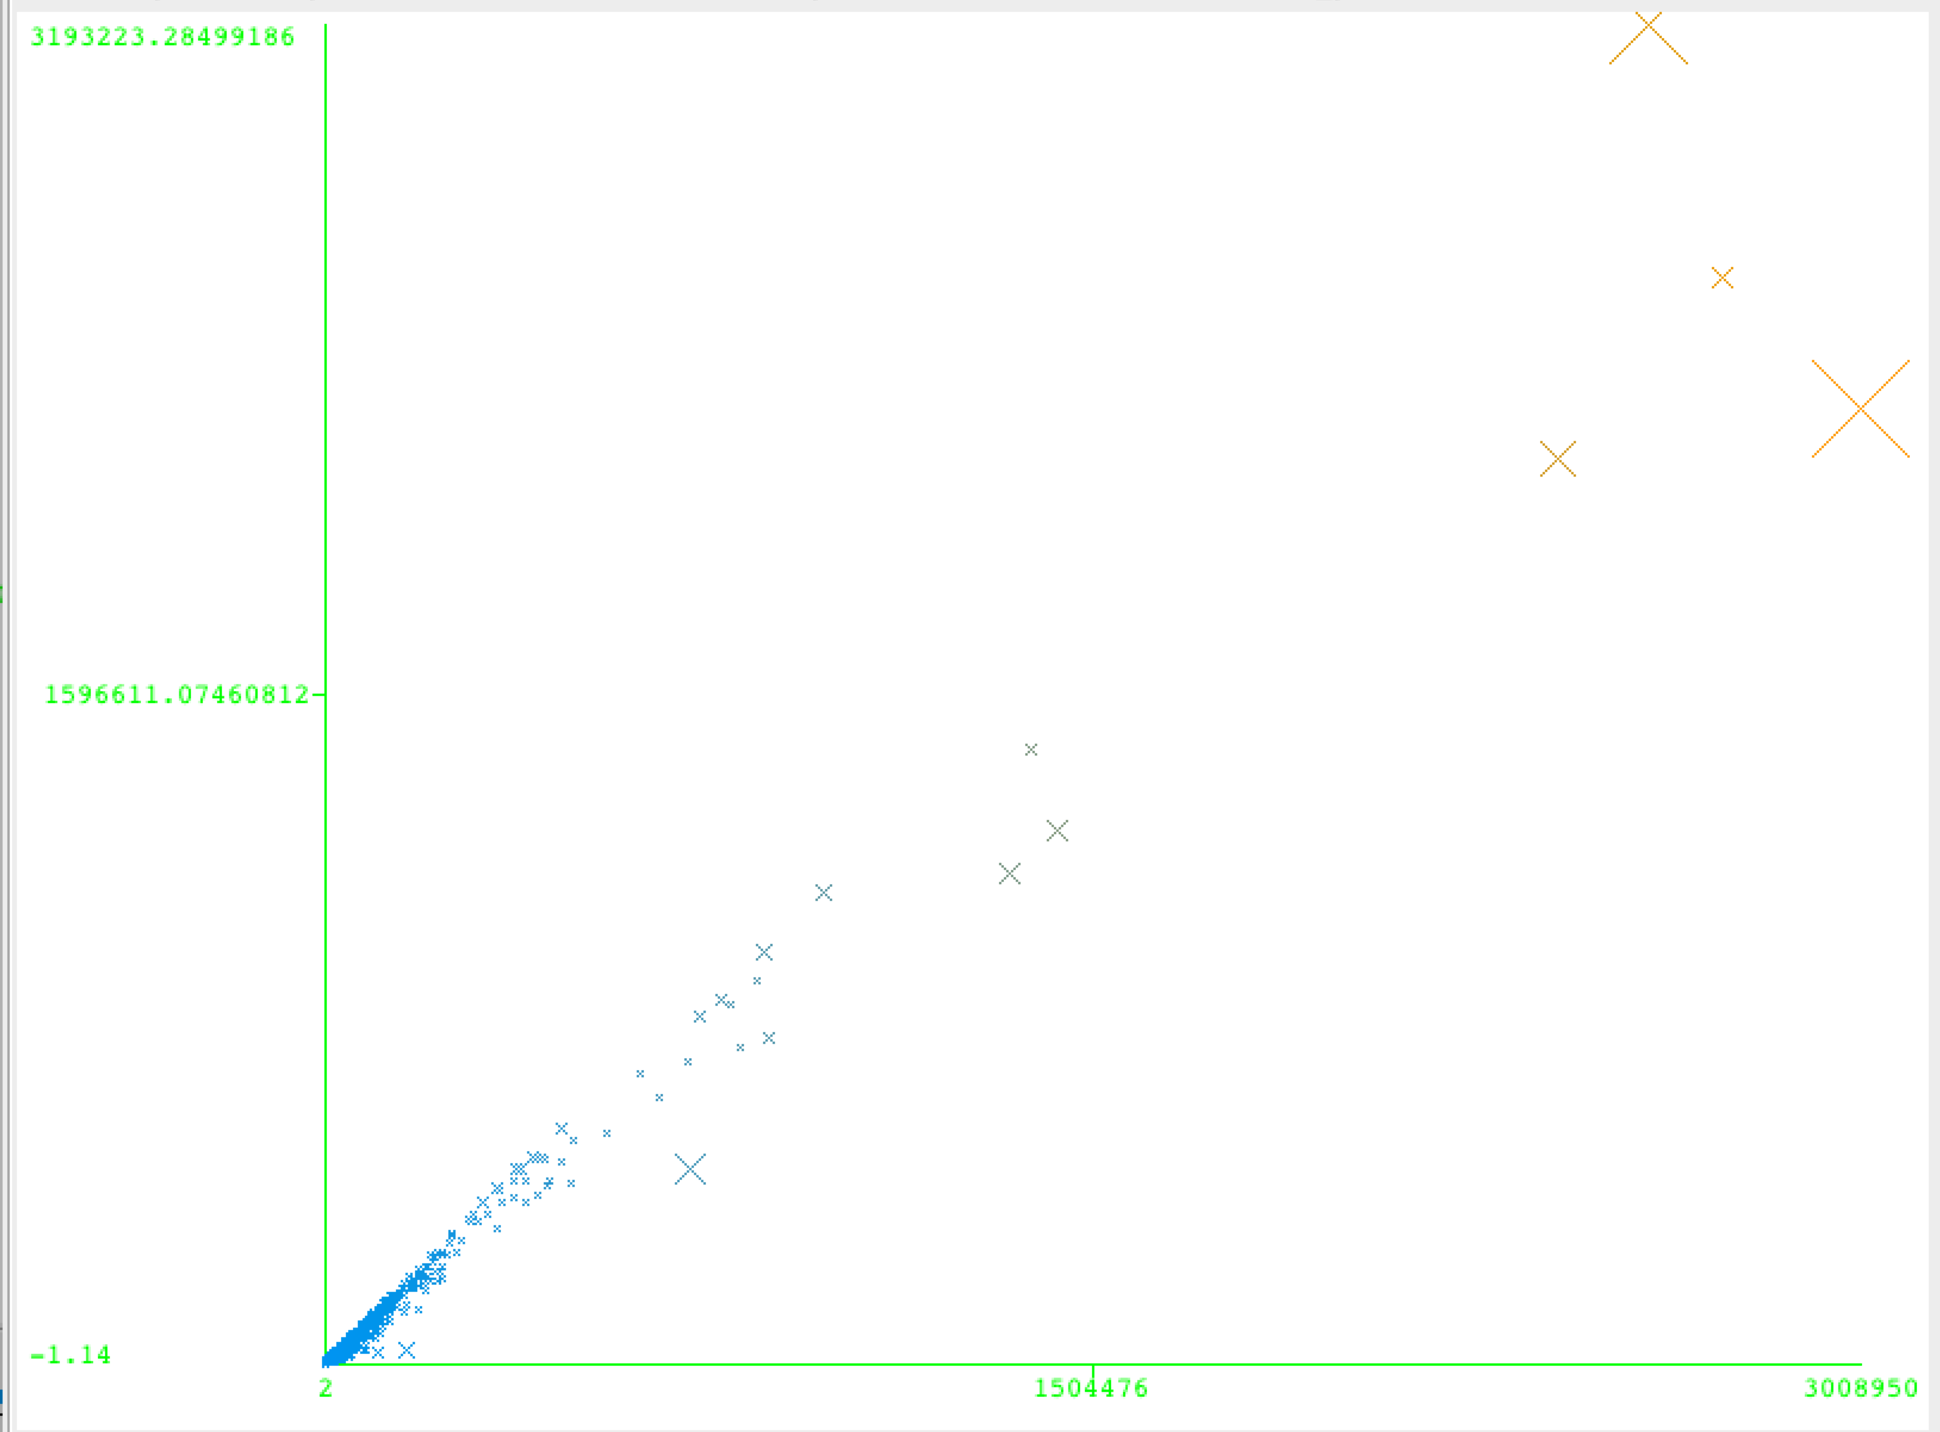
\includegraphics[width=3.5in, keepaspectratio = true]{neditserrors.png}
\caption*{(a) Outliers in the nedit/narticles model.}
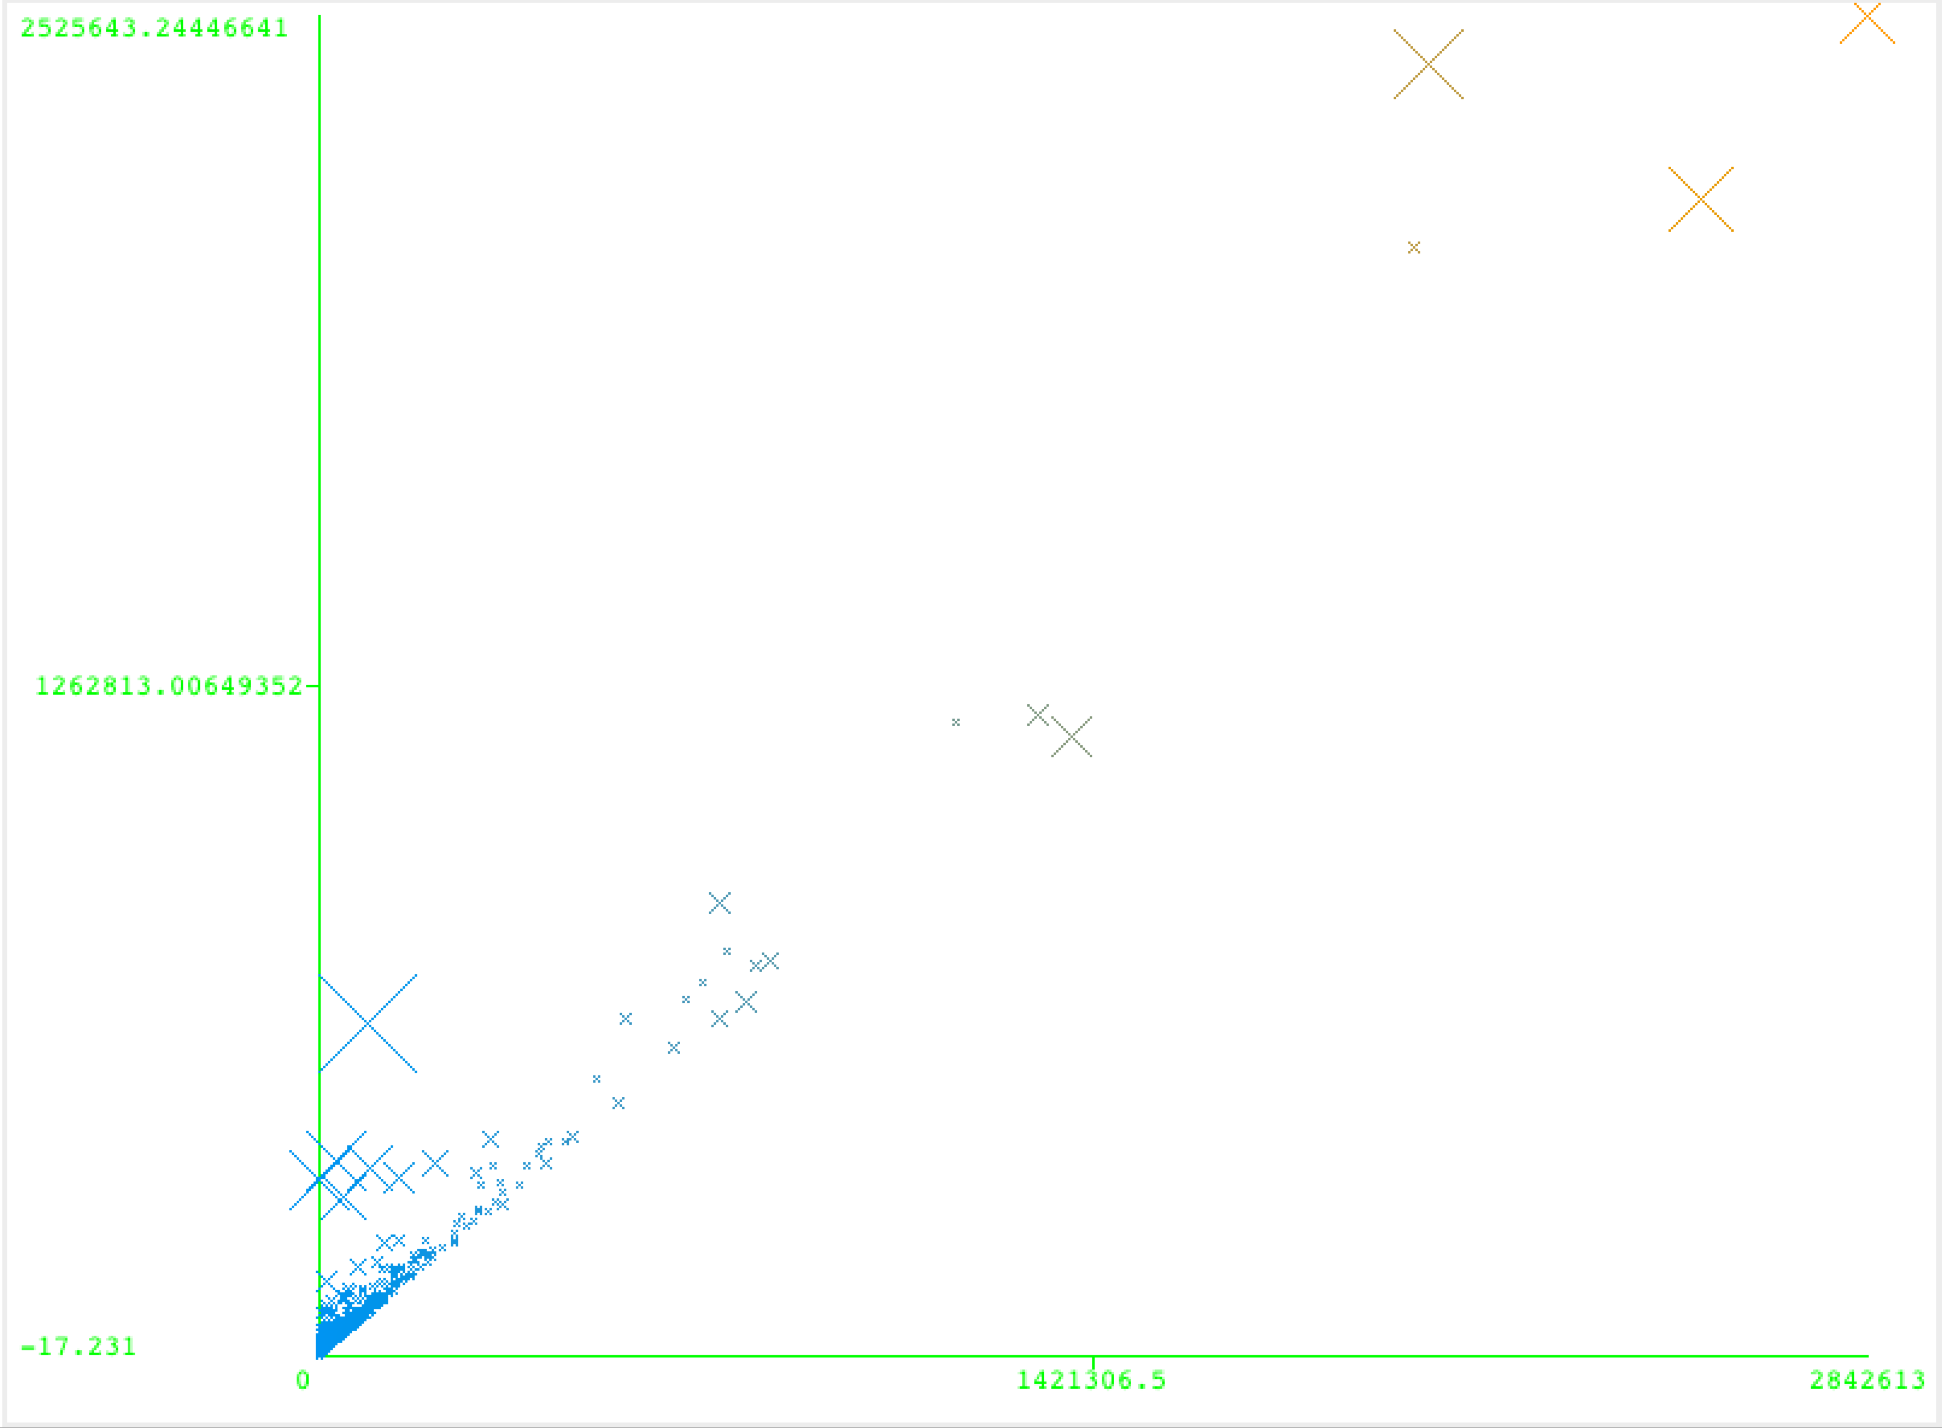
\includegraphics[width=3.5in, keepaspectratio = true]{articlenseditserrors.png}
\caption*{(b) Outliers in the nsarticleedits/edits modeleee.}
\caption{}
\label{outliers}
\end{figure}

\subsection{Evaluating User Model}
\subsubsection{Precision - Recall for Bots}

In order to evaluate the effectiveness of each outlier measure we compared five different rankings of users:
\begin{enumerate}
\item Outlier score (\textbf{score}) - Using the LB/UB bounds, score a point to each user profile for a violation of any number of bounds. Rank users by points. (Users with 0 points are ranked arbitrarily following users with non-zero points.)
\item Raw Edit count (\textbf{edits}) - Rank users by nedits variable.
\item nsarticleedits/nedits model error (\textbf{articlens-error}) - Rank users by the difference between actual and predicted value.
\item nedits/narticles model error (\textbf{nedits-error}) - Rank users by the difference between actual and predicted value.
\item pctnsadminedits/pctnsarticleedits model error (\textbf{pctadmin-error}) - Rank users by the percentage difference between actual and predicted value.
\end{enumerate}

In Figure \ref{prec} we evaluate each score using a precision-recall curve for each of the five scores, using the rough criteria that any profile that matches ``bot'' (non-case sensitive) is a positive result. For low recall levels, the \textbf{artclens-error} and \textbf{nedits-error} have high precision, with an interesting initial blip in the \textbf{pctadmin-error} curve. Suprisingly, one of the worst performing measures is the combined outlier score. Raw edit count alone outperforms the combined outlier score.

\begin{figure}
\centering
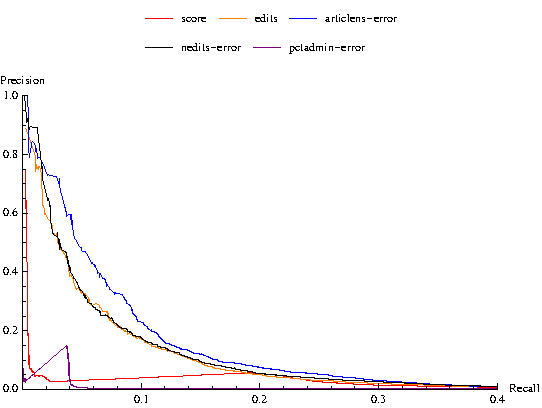
\includegraphics[width=4.5in, keepaspectratio = true]{precisionrecall.pdf}
\caption{Precision Recall for profile scores.}
\label{prec}
\end{figure}

\subsubsection{Manual Evaluation}

To better evluate the performance of each score we manually examined the top scoring user accounts by each score.

\begin{landscape}
\begin{table}
\begin{center}
\tiny
\begin{tabular}{l}
\hline
Outlier \\
\hline
MiszaBot I \\
AlexNewArtBot \\
West.andrew.g \\
COIBot \\
Mathbot \\
Athaenara \\
Scsbot \\
MiszaBot II \\
Mikhailov Kusserow \\
WP 1.0 bot \\
EmanWilm \\
Ahnoneemoos \\
Werdnabot \\
WLU \\
Xn4 \\
Cyde \\
Scott MacDonald \\
Sango123 \\
RickK \\
Pcap \\
MiszaBot III \\
Makemi \\
La Pianista \\
Joseph A. Spadaro \\
Hasteur \\
GuillaumeTell \\
Evanh2008 \\
Tryptofish \\
Doc glasgow \\
Bobblehead \\
Andrewa \\
03md \\
Zad68 \\
SwisterTwister \\
Steven J. Anderson \\
Spartaz \\
SharedIPArchiveBot \\
PumpkinSky \\
Proofreader77 \\
Pomte \\
Swatjester \\
PCHS-NJROTC \\
Oneiros \\
Nsk92 \\
Largoplazo \\
Jax 0677 \\
Geometry guy \\
FF2010 \\
Enigmaman \\
\end{tabular}
\begin{tabular}{l} 
\hline
 Edit Count \\
\hline
SmackBot \\
Yobot \\
Addbot \\
Cydebot \\
ClueBot NG \\
RjwilmsiBot \\
EmausBot \\
Koavf \\
ClueBot \\
RussBot \\
Xqbot \\
Luckas-bot \\
Waacstats \\
Rich Farmbrough \\
Lightbot \\
SineBot \\
AnomieBOT \\
The Anomebot2 \\
ZéroBot \\
Rjwilmsi \\
FrescoBot \\
TXiKiBoT \\
Woohookitty \\
Helpful Pixie Bot \\
Tassedethe \\
Bearcat \\
ListasBot \\
Legobot \\
Thijs!bot \\
SporkBot \\
Erik9bot \\
BetacommandBot \\
VolkovBot \\
Fbot \\
BOTijo \\
Kingbotk \\
Ser Amantio di Nicolao \\
Hmains \\
D6 \\
Xenobot Mk V \\
Alaibot \\
SieBot \\
BD2412 \\
Full-date unlinking bot \\
XLinkBot \\
Bluebot \\
AvicBot \\
Magioladitis \\
BattyBot \\
\end{tabular}
\begin{tabular}{l}
\hline
Nsarticleedits error \\
\hline 
SineBot \\
Yobot \\
ListasBot \\
Kingbotk \\
BetacommandBot \\
Xenobot Mk V \\
Fbot \\
Erik9bot \\
MiszaBot III \\
Koavf \\
Skier Dude \\
WOSlinker \\
TXiKiBoT \\
MartinBotIII \\
EdwardsBot \\
Reedy Bot \\
Cydebot \\
BotMultichill \\
TinucherianBot \\
SatyrBot \\
OrphanBot \\
AnomieBOT \\
ShepBot \\
DASHBot \\
Bhadani \\
DodoBot \\
Sfan00 IMG \\
Kumi-Taskbot \\
John Carter \\
OOODDD \\
MiszaBot I \\
VolkovBot \\
Gene93k \\
MGA73bot \\
AnnaKucsma \\
PhotoCatBot \\
Escarbot \\
BJBot \\
TonyTheTiger \\
STTWbot \\
MetsBot \\
DPL bot \\
MiszaBot II \\
Wizardman \\
FairuseBot \\
Merenta \\
Rettetast \\
Epbr123 \\
LaraBot \\
\end{tabular}
\begin{tabular}{l}
\hline
 Nedits error \\
\hline
SmackBot \\
Addbot \\
Cydebot \\
SineBot \\
EmausBot \\
ClueBot NG \\
Yobot \\
Koavf \\
MiszaBot III \\
RussBot \\
Helpful Pixie Bot \\
ClueBot \\
Lightbot \\
BOTijo \\
Rich Farmbrough \\
Erik9bot \\
EdwardsBot \\
Fbot \\
RjwilmsiBot \\
Alaibot \\
Full-date unlinking bot \\
SporkBot \\
ZéroBot \\
Xenobot Mk V \\
Legobot \\
Ser Amantio di Nicolao \\
AvicBot \\
Xqbot \\
Waacstats \\
BattyBot \\
Luckas-bot \\
Kingbotk \\
Escarbot \\
VIAFbot \\
Eubot \\
TXiKiBoT \\
MiszaBot I \\
ListasBot \\
Magioladitis \\
BG19bot \\
Vsmith \\
FrescoBot \\
ChrisGualtieri \\
WOSlinker \\
Ksnow \\
Bgwhite \\
Bluebot \\
BD2412 \\
Kwamikagami \\
\end{tabular}
\begin{tabular}{l}
\hline
pctnsadminedits error \\
\hline 
Jph0917 \\
MikeWattHCP \\
Sierra2008 \\
Kevinsam \\
MystBot \\
XxXDylanWillard \\
Brf1000 \\
Dan1216 \\
GundersonM \\
Chongkian \\
Ddrane \\
Kai662 \\
Ps07swt \\
LtMuldoon \\
Native truth \\
Manushand \\
Hup234 \\
Zgystardst \\
Fifties \\
Antlersantlers \\
Raulsebrook \\
CN3777 \\
MC32 \\
Kippi70 \\
Kwellyn \\
Eloewien \\
Enbionycacruz \\
Bororule12 \\
Quebec99 \\
Thom2729 \\
My Ovation \\
JohnSawyer \\
VsBot \\
Ldaniel77 \\
Viva britney \\
Johnny longtorso \\
Historynut101 \\
Cyanolinguophile \\
Danicalove79 \\
Na zdravy \\
The Brain of Pooh \\
Eustanacio IV \\
Midnight man \\
Gpath1k \\
Wukai \\
BrightStarSky \\
Huskertsd \\
Filippos Greece \\
Ronmore \\
\end{tabular}
\label{scorechart}
\caption{Top scoring users for each ranking scheme}
\end{center}
\end{table}
\end{landscape}

\subsection{User co-edit network Visualization}

After processing the revision metadata the graph includes 26251504 edges. Filtering out edges of weight 1 leaves 2611449 edges. How many nodes? Results from Weight distribution, degree centrality and weighted degree centrality.

Using Gephi to visualize. Might make sense to program some sort of centrality measures (e.g. degree centrality) outside of Gephi because they will scale better.

\section{Discussion}
\subsection{Success?}
Were the hypotheses validated? Manually inspect users to see if they actually correspond to spammers and bots.
%    Discussion - interpret the results and make generalizations and broader lessons
\subsection{Limitations}
What were some of the limitations? What are the opportunities for future work?
\begin{itemize}
\item With more time there would be more opportunities to validate results better, form better hypotheses using manual analysis.
\end{itemize}
\section{Conclusions}
\section{Reference}
Figure out this bibtex thing.
\end{document}



%\begin{itemize}
%\item Using outliers of the distributions of each variable, we identify 68411 with at least one outlier field. And 931427 without. Of the outlier set 832 (0.01216178684714) have account names matching ``bot'', of the non-outlier set there are 1798 (0.00193037135492).
%\end{itemize}


%% \begin{verbatim}

%% {{"id", 0}, {"nedits", 2}, {"narticles", 1}, {"daysactive", 
%%   2}, {"naddedits", 0}, {"nremoveedits", 0}, {"bytesadded", 
%%   0}, {"bytesremoved", 0}, {"avgeditsday", 0.0004}, {"avgarticlesday",
%%    0.0002}, {"avgtimetonext", 0.}, {"avgbytesadded", 
%%   0}, {"avgbytesremoved", 
%%   0}, {"netbytes", -11423784}, {"avgnetbytes", -95917.3}, \
%% {"articlensedits", 0}, {"adminnsedits", 0}, {"pctarticlensedits", 
%%   0}, {"pctadminnsedits", 0}}

%% {{"id", 999835}, {"nedits", 3008950}, {"narticles", 
%%   2504647}, {"daysactive", 4571}, {"naddedits", 
%%   2949526}, {"nremoveedits", 135820}, {"bytesadded", 
%%   1793038869}, {"bytesremoved", 301961193}, {"avgeditsday", 
%%   1486.02}, {"avgarticlesday", 1311.33}, {"avgtimetonext", 
%%   3633.5}, {"avgbytesadded", 2.40006*10^6}, {"avgbytesremoved", 
%%   1.26337*10^6}, {"netbytes", 1790307455}, {"avgnetbytes", 
%%   2.40006*10^6}, {"articlensedits", 2842613}, {"adminnsedits", 
%%   683585}, {"pctarticlensedits", 1}, {"pctadminnsedits", 1}}


%% === Run information ===

%% Scheme:weka.classifiers.functions.LinearRegression -S 0 -R 1.0E-8
%% Relation:     wikiprofile.noip.nohist.vector-weka.filters.unsupervised.attribute.Remove-R4-15
%% Instances:    999836
%% Attributes:   3
%%               id
%%               nedits
%%               narticles
%% Test mode:10-fold cross-validation

%% === Classifier model (full training set) ===


%% Linear Regression Model

%% nedits =

%%       1.2311 * narticles +
%%       3.5835

%% Time taken to build model: 1.67 seconds

%% === Cross-validation ===
%% === Summary ===

%% Correlation coefficient                  0.986 
%% Mean absolute error                     33.47  
%% Root mean squared error               1208.4059
%% Relative absolute error                 10.0365 %
%% Root relative squared error             16.7038 %
%% Total Number of Instances           999836     

%% === Run information ===

%% Scheme:weka.classifiers.functions.LinearRegression -S 0 -R 1.0E-8
%% Relation:     wikiprofile.noip.vector-weka.filters.unsupervised.attribute.Remove-R2-17
%% Instances:    999836
%% Attributes:   3
%%               id
%%               pctarticlensedits
%%               pctadminnsedits
%% Test mode:10-fold cross-validation

%% === Classifier model (full training set) ===


%% Linear Regression Model

%% pctadminnsedits =

%%      -0.8621 * pctarticlensedits +
%%       0.8579

%% Time taken to build model: 2.82 seconds

%% === Cross-validation ===
%% === Summary ===

%% Correlation coefficient                  0.9164
%% Mean absolute error                      0.0405
%% Root mean squared error                  0.0943
%% Relative absolute error                 22.9393 %
%% Root relative squared error             40.0244 %
%% Total Number of Instances           999836     

%% === Run information ===

%% Scheme:weka.classifiers.functions.LinearRegression -S 0 -R 1.0E-8
%% Relation:     wikiprofile.noip.vector-weka.filters.unsupervised.attribute.Remove-R3-15,17-19
%% Instances:    999836
%% Attributes:   3
%%               id
%%               nedits
%%               articlensedits
%% Test mode:10-fold cross-validation

%% === Classifier model (full training set) ===


%% Linear Regression Model

%% articlensedits =

%%       0.8607 * nedits +
%%     -12.0717

%% Time taken to build model: 1.63 seconds

%% === Cross-validation ===
%% === Summary ===

%% Correlation coefficient                  0.9815
%% Mean absolute error                     35.0435
%% Root mean squared error               1211.6506
%% Relative absolute error                 13.2126 %
%% Root relative squared error             19.1423 %
%% Total Number of Instances           999836     
%% \end{verbatim}

